\documentclass[aspectratio=43]{beamer}
\usepackage[english]{babel}
\usepackage{amsthm}
\usepackage{mathtools}
\usepackage{physics}
\usepackage{calligra}
\usepackage{csquotes}
\usepackage{tensor}
\usepackage[thicklines]{cancel}
\usepackage{tcolorbox}
\usepackage{pstricks}
\usepackage{setspace}
\usepackage[backend=biber, bibstyle=nature, sorting=nty, citestyle=numeric-comp]{biblatex} %Custom bibliography
    \addbibresource{bib.bib} %Load references


\DeclareMathAlphabet{\mathcalligra}{T1}{calligra}{m}{n}
\DeclareFontShape{T1}{calligra}{m}{n}{<->s*[2.2]callig15}{}
\newcommand{\scriptr}{\mathcalligra{r}\,}
\newcommand{\boldscriptr}{\pmb{\mathcalligra{r}}\,}
\def\rc{\scriptr}
\def\brc{\boldscriptr}
\def\hrc{\hat\brc}
\newcommand{\ie}{\emph{i.e.}} %id est
\newcommand{\eg}{\emph{e.g.}} %exempli gratia
\newcommand{\rtd}[1]{\ensuremath{\left\lfloor #1 \right\rfloor}}
\newcommand{\dirac}[1]{\ensuremath{\delta \left( #1 \right)}}
\newcommand{\diract}[1]{\ensuremath{\delta^3 \left( #1 \right)}}
\newcommand{\e}{\ensuremath{\epsilon_0}}
\newcommand{\m}{\ensuremath{\mu_0}}
\newcommand{\V}{\ensuremath{\mathcal{V}}}
\newcommand{\prnt}[1]{\ensuremath{\left(#1\right)}} %parentheses
\newcommand{\colch}[1]{\ensuremath{\left[#1\right]}} %square brackets
\newcommand{\chave}[1]{\ensuremath{\left\{#1\right\}}}  %curly brackets

\useoutertheme{infolines}
\useinnertheme{rectangles}
\usefonttheme{professionalfonts}


\definecolor{orange}{HTML}{f28165}
\definecolor{gray}{HTML}{303030}
\definecolor{yellow}{HTML}{f0be52}
\definecolor{lightorange}{HTML}{f19e58}

\renewcommand{\CancelColor}{\color{orange}}

\makeatletter
\newcommand{\mybox}[1]{%
  \setbox0=\hbox{#1}%
  \setlength{\@tempdima}{\dimexpr\wd0+13pt}%
  \begin{tcolorbox}[colback=orange,colframe=orange,boxrule=0.5pt,arc=4pt,
      left=6pt,right=6pt,top=6pt,bottom=6pt,boxsep=0pt,width=\@tempdima]
    \textcolor{white}{#1}
  \end{tcolorbox}
}
\makeatother

\usecolortheme[named=orange]{structure}
\usecolortheme{sidebartab}
\usecolortheme{orchid}
\usecolortheme{whale}
\setbeamercolor{alerted text}{fg=yellow}
\setbeamercolor{block title alerted}{bg=alerted text.fg!90!black}
\setbeamercolor{block title example}{bg=lightorange!60!black}
\setbeamercolor{background canvas}{bg=gray}
\setbeamercolor{normal text}{bg=gray,fg=white}

\setbeamertemplate{footline}
        {
      \leavevmode%
      \hbox{%
      \begin{beamercolorbox}[wd=.25\paperwidth,ht=2.25ex,dp=1ex,center]{author in head/foot}%
        \usebeamerfont{author in head/foot}\insertshortauthor~~(\insertshortinstitute)
      \end{beamercolorbox}%
      \begin{beamercolorbox}[wd=.25\paperwidth,ht=2.25ex,dp=1ex,center]{title in head/foot}%
        \usebeamerfont{title in head/foot}\insertshorttitle
      \end{beamercolorbox}%
      \begin{beamercolorbox}[wd=.25\paperwidth,ht=2.25ex,dp=1ex,center]{date in head/foot}%
        \usebeamerfont{date in head/foot}\insertshortdate{}%\hspace*{2em}

      \end{beamercolorbox}

      \begin{beamercolorbox}[wd=.25\paperwidth,ht=2.25ex,dp=1ex,center]{date in head/foot}%
        % \usebeamerfont{date in head/foot}\insertshortdate{}%\hspace*{2em}
        %
      %#turning the next line into a comment, erases the frame numbers
        \insertframenumber{} / \inserttotalframenumber
        % \hspace*{2ex}
      \end{beamercolorbox}}%
      \vskip0pt%
    }


\setbeamertemplate{blocks}[rectangle]
\setbeamercovered{dynamic}

\setbeamertemplate{section page}
{
	\begin{centering}
		\begin{beamercolorbox}[sep=27pt,center]{part title}
			\usebeamerfont{section title}\insertsection\par
			\usebeamerfont{subsection title}\insertsubsection\par
		\end{beamercolorbox}
	\end{centering}
}

%\setbeamertemplate{subsection page}
%{
%	\begin{centering}
%		\begin{beamercolorbox}[sep=12pt,center]{part title}
%			\usebeamerfont{subsection title}\insertsubsection\par
%		\end{beamercolorbox}
%	\end{centering}
%}

\newcommand{\hlight}[1]{\colorbox{violet!50}{#1}}
\newcommand{\hlighta}[1]{\colorbox{red!50}{#1}}

\title{***} %->->->->-> Check hyperref title <-<-<-<-<-
\subtitle{**}
\author[LI]{LI $\cdot$ Zikang}
\institute[HKUST]{
    IEDA%
    \\%
    The Hong Kong University of Science and Technology%
} %You can change the Institution if you are from somewhere else
\date{}

\begin{document}
    \frame{\titlepage}
    \begin{frame}{Table of contents}
        \tableofcontents
    \end{frame}

    % !TeX root = ../main.tex

\section{Dynamic Model}
    \frame{\sectionpage}

    \begin{frame}
        \centering
        % \begin{equation*}
        %     V_{t}(x) = E\left[\max_{u \in \{0,1\}} \{R u + V_{t+1}(x- S u)\}\right]\end{equation*}
        % \end{equation*}
          \begin{equation*}
            V_{t}(x) = \sum_{i} \lambda_i \left[\max_{u \in \{0,1\}}\{s_i u + V_{t+1}(x- (1+s_i) u)\}  \right] + (1-\sum_i \lambda_i)V_{t+1}(x)
          \end{equation*}
             \begin{equation*}
               = \sum_{i} \lambda_i \left[\max\{s_i + V_{t+1}(x-1-s_i),V_{t+1}(x)\}\right] + (1-\sum_i \lambda_i)V_{t+1}(x)
             \end{equation*}
             \begin{equation*}
               = V_{t+1}(x) + \sum_{i} \lambda_i \left[\max\{s_i + V_{t+1}(x-1-s_i)-V_{t+1}(x),0\}\right]
             \end{equation*}
    \end{frame}

    \begin{frame}
      \begin{itemize}
        \item $x$, remaining capacity.
        \vspace{10pt}
        % \item $R,S$, random variable.
        % \vspace{10pt}
        \item $s_i$, the number of people $i$th type of group contains. If we suppose the number is continuous, then $s = \{1, \ldots,n\}$.
        \vspace{10pt}
        \item $\lambda_i$: the probability of an arrival of $s_i$.
        \vspace{10pt}
        \item $u$, binary variable. $u=1$, accept.
      \end{itemize}
    \end{frame}

    \begin{frame}{Properties of marginal value}
      \begin{itemize}
        \item $f(x) = \max_{a =\{0,1\}} \{a(p-1) +g(x-ap)\}$, $p = s_i +1 > 0, a = u$.
        \item $f(x) = V_t(x)$, $g(x) = V_{t+1}(x)$.
        \vspace{10pt}
        \item $f(x)$ is not concave means the marginal values $\Delta V_j(x)$ is not decreasing in the remaining capacity at a given stage $j$, is not increasing in the number of stages remaining at a given capacity level $x$.
        \vspace{10pt}
        \item $V_{t+2}(x-s_i-1)-V_{t+1}(x-s_i-1) \leq V_{t+2}(x)-V_{t+1}(x) \Rightarrow V_{t}(x) - V_{t+1}(x) \geq V_{t+1}(x) -V_{t+2}(x)$.
        \vspace{10pt}
        \item Only have $V_t(x) \geq V_{t+1}(x)$, $V_t(x) \leq V_t(x+1)$.
        \item No general rules.
      \end{itemize}
    \end{frame}

    \begin{frame}{Our model}
      \begin{equation*}
          V_{t}(x) = V_{t+1}(x) + \sum_{i} \lambda_i \left[\max\{s_i + V_{t+1}(x-1-s_i)-V_{t+1}(x),0\}\right]
        \end{equation*}

        \vspace{10pt}
        \centering
        Let $\Delta_i V_{t+1}(x) = V_{t+1}(x) - V_{t+1}(x-1-s_i)$

        \vspace{20pt}

        To accept $s_i$ means $s_i \geq \Delta_i V_{t+1}(x)$.

        To reject $s_i$ means $s_i < \Delta_i V_{t+1}(x)$.
    \end{frame}

    \begin{frame}{Some corollaries}
      \begin{itemize}
        \justifying
        \item If $s_i=k$ is accepted, we will accept $s_i=k+1$ only when $1 \geq V_{t+1}(x-1-s_i) - V_{t+1}(x-2-s_i)$.
        \item If $s_i=k$ is rejected, we will reject $s_i=k-1$ only when $1 \geq V_{t+1}(x-s_i)- V_{t+1}(x-1-s_i)$.
        \vspace{10pt}
        \item Fix some stage, when remaining seats $\to \infty$, the decision is to accept all groups of different sizes.
        \vspace{10pt}
        \item $E_T$ denotes the convergence value at the last stage, which equals to the expectation of $s_i$, i.e. $E_T = E(s)$. $s_i$ is the number of people in a group.
        \vspace{10pt}
        \item $E_t = (T-t+1) E_T$. $S_t$ denotes the number of remaining seats when $V_t(x)$ converges for the first time at stage $t$, then $S_{t-1}$ is at most $S_t + (\max\{s_i\}+1)$. That is, the period is $\max\{s_i\}+1$.
      \end{itemize}
    \end{frame}

    \begin{frame}{Explanation}
      \begin{itemize}
        \item When $s_i \geq V_{t+1}(x) - V_{t+1}(x-1-s_i)$, then $s_i+1 \geq V_{t+1}(x) - V_{t+1}(x-1-s_i)+1 \geq V_{t+1}(x) - V_{t+1}(x-2-s_i)$, the latter inequality holds because one seat can only provide at most one unit of value. That is,
        $1 \geq V_{t+1}(x-1-s_i) - V_{t+1}(x-2-s_i)$.
        \vspace{10pt}
        \item Similarly, because $V_{t+1}(x-s_i) \leq  V_{t+1}(x-1-s_i)+1$, $s_i-1 \leq V_{t+1}(x) - V_{t+1}(x-1-s_i)-1 \leq V_{t+1}(x) - V_{t+1}(x-s_i)$
        \vspace{10pt}
        \item Fix the last stage, it is clear that when remaining seats are large enough, the convergence value of $V_T(x)$ will be $E_T = E(s)$ because we will accpet any group.
      \end{itemize}
    \end{frame}

    \begin{frame}{A special case}
      \begin{itemize}
        \item For the case that we only have $\{1,2\}$ people in a group.
        \item For $V_t(3)$, always reject $1$; For $V_t(2)$, always reject $2$.
        \item For $V_t(s), s=4,5$, we will always accept $\{1,2\}$ when $\lambda_1 \geq \lambda_2$.
        \item For $V_t(s), s \geq 6$, this policy is invalid.
        \item But $V_t(x) \leq V_t(x-1) +1$ always holds, for any $x>1$ when given any stage $t$.
        \item $V_t(3) - V_t(2) \leq 1, V_t(2) - V_t(1) \leq 1 \Rightarrow V_{t-1}(5) - V_{t-1}(4) \leq 1$.
        \item To prove $t$ at first, then prove $s$.
        % \item $V_t(s-2) - V_t(s-3) \leq 1, V_t(s-3) - V_t(s-4) \leq 1 \Rightarrow V_{t-1}(s) - V_{t-1}(s-1) \leq 1$.
      \end{itemize}
    \end{frame}

    \begin{frame}{Proof}
      When $\lambda_1 \geq \lambda_2$.
      \begin{itemize}
        \item Periodicity

        $1 + V_t(3n+1) < V_t(3n+3), t<T_0.$
        $1 + V_t(3n) \geq V_t(3n+2), 1 + V_t(3n-1) \geq V_t(3n+1)$.

        \item Under the assumption, show $V_t(3n+1)-V_t(3n) \leq 1$, $V_t(3n+2)-V_t(3n+1) \leq 1$ and $V_t(3n+3)-V_t(3n+2) \leq 1$ respectively.

        % \item  To extend our conclusion, when $\lambda_1 > \lambda_2> \ldots > \lambda_n,
        % V_t(x) \leq V_t(x-1) +1$, for any $x>1$ when given any stage $t$.
        \item $V_{t-1}(x) - V_{t}(x)\geq V_{t-1}(x-s-1) - V_{t}(x-s-1) \Rightarrow$
        $V_t(x) \leq V_t(x-s-1) +s$ always holds. $s = \max\{s_i\}$.
      \end{itemize}
    \end{frame}

    \begin{frame}{Some Notes}
      \begin{itemize}
        \item At first, $\lambda_1 \geq \lambda_2 \Rightarrow V_T(3) \leq V_T(2) +1 \Rightarrow V_t(3) \leq V_t(2) +1 $.
        \item Similarly, we have $V_t(4) \leq V_t(3) +1, V_t(5) \leq V_t(4) +1$.
        \item In order to prove that $V_t(x) \leq V_t(x-1) +1$, we have to make sure whether we reject $\{1\}$ first.
        \item $V_{T-1}(6) \leq V_{T-1}(4) +1$ needs $\lambda_1^2 \geq \lambda_2 \Rightarrow \lambda_2 \leq \frac{3- \sqrt{5}}{2}.$
        \item Fix $s_i$, $\Delta_i V_t(x+1) \leq \Delta_i V_t(x)$ and $\Delta_i V_{t+1}(x) \leq \Delta_i V_t(x)$ do not hold.
      \end{itemize}
    \end{frame}

    \begin{frame}{Notation Description}
      \begin{itemize}
        \justifying
        \item $S$ State: Remaining seats.
        \vspace{10pt}
        \item $a$ Action: Accept,1 or Reject,0.
        \vspace{10pt}
        \item $T$ Stage: $|T|$ The remaining number of groups need to be served.
        \vspace{10pt}
        \item $V(S,T)$: Value function at state $S$ in stage $T$.
        \vspace{10pt}
        \item Reward(value at each stage): $|s_i|$ The number of people the current group contains.
      \end{itemize}
    \end{frame}


    \begin{frame}{Bellman equation}
      \begin{itemize}
        \item When $T > 1$
      \end{itemize}

      $$V(S,T) = \sum_{i \in N} p_i \max\{ {[V((S-s_i-1),T-1)+ s_i]}, {V(S,T-1)} \}$$

      \begin{itemize}
        \item When $T = 1$
      \end{itemize}

      $$V(S,1) = \sum_{i \in N}p_i \max\{ {[V((S-s_i),0)+ s_i]}, {V(S,0)} \}$$

      \vspace{10pt}
      $S$ remaining seats and $T$ remaining stages.

      Explanation: At the last stage, no need to leave space.
    \end{frame}

    \begin{frame}{Boundary conditions}
      \begin{itemize}
        \item When $t \geq 0$
      \end{itemize}

      \begin{equation*}
      \mathrm{V}(\mathrm{k}, \mathrm{t})=\left\{\begin{array}{c}
      -\infty, k<0 \\
      0,~ k=0
      \end{array} \right. \\
    \end{equation*}

      \begin{itemize}
        \item When $t = 0$
      \end{itemize}

      \begin{equation*}
        \mathrm{V}(\mathrm{k}, \mathrm{t})=0, \mathrm{k}>0
      \end{equation*}

    \end{frame}

    \begin{frame}{An example}
      Suppose that the groups $s_i, i\in N$ satisfy a certain distribution. For example, a fixed discrete distribution.

      \begin{table}[]
      \begin{tabular}{lllll}
      $s_i$ & 1   & 2   & 3   & 4   \\
      $p_i$ & 0.2 & 0.2 & 0.3 & 0.3
      \end{tabular}
      \end{table}
      \vspace{10pt}
      Let $S=14, T=5$, then we have
      \begin{align*}
      V(14,5) = 0.2[\max\{V(12,4)+1,V(14,4)\}] \\+ 0.2[\max\{V(11,4)+2, V(14,4) \}] \\+ 0.3[\max\{V(10,4)+3, V(14,4)\}] \\+ 0.3[\max\{ V(9,4)+4, V(14,4)\}]
      \end{align*}
      $$\cdots$$
    \end{frame}

    \begin{frame}{Result}
      \centering
      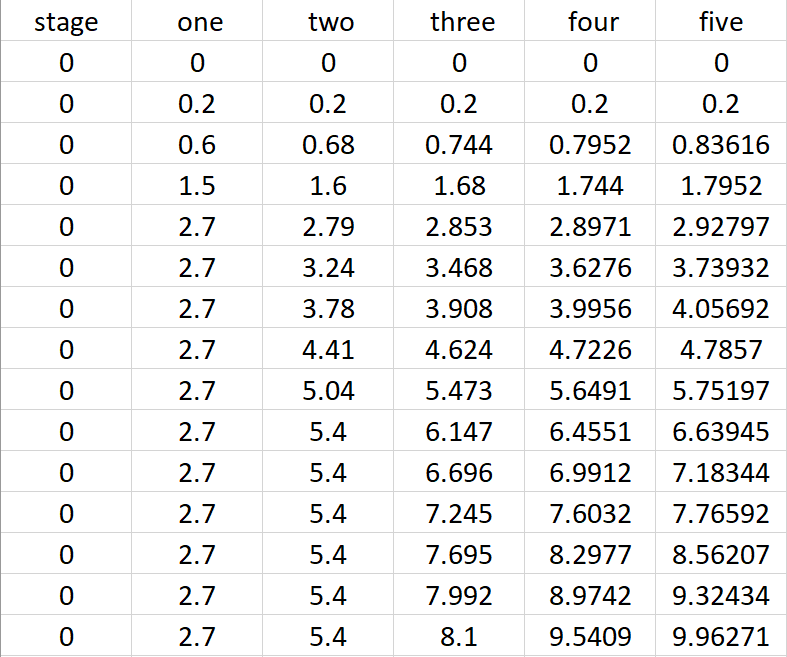
\includegraphics[width = 0.7\textwidth]{images/result1}
    \end{frame}

    % \begin{frame}{Extension}
    %
    % \end{frame}

    % !TeX root = ../main.tex

\section{Seat Planning with Deterministic Demand}
    \frame{\sectionpage}

  \begin{frame}{Deterministic Formulation}  %开始一张幻灯片
    Seat planning problem with given demand $\bm{d}$:

    \begin{equation}\label{deter_upper}
      \begin{aligned}
      \max \quad & \sum_{i=1}^{M}  \sum_{j= 1}^{N} (n_i- \delta) x_{ij} \\
      \text {s.t.} \quad & \sum_{j= 1}^{N} x_{ij} \leq d_{i}, \quad i \in \mathcal{M}, \\
      & \sum_{i=1}^{M} n_{i} x_{ij} \leq L_j, j \in \mathcal{N}, \\
      & x_{ij} \in \mathbb{Z}_{+}, \quad i \in \mathcal{M}, j \in \mathcal{N}.
      \end{aligned}
    \end{equation}
    Objective: maximize the number of people accommodated.

    $x_{ij}$: the number of group type $i$ in row $j$.
  \end{frame}

  \begin{frame}{Property}
    In the LP relaxation of problem \eqref{deter_upper}, there exists an index $v$ such that the optimal solutions satisfy the following conditions:

    \begin{itemize}
      \item For $i = 1,\ldots, v-1$ and for all $j$, $x_{ij}^{*} = 0$. 
      % indicating that no group type $i$ are assigned to any rows before index $v$.
      \item For $i = v+1,\ldots, M$, $\sum_{j} x_{ij}^{*} = d_{i}$. 

      \item For $i = v$, $\sum_{j} x_{ij}^{*} = \frac{L - \sum_{i = v+1}^{M} {d_i n_i}}{n_v}$ 
      % This quantity is determined by the available supply, which is calculated as the remaining seats after accommodating the demands for group types $v+1$ to $M$, divided by the size of group type $v$, denoted as $n_v$.
    \end{itemize}

    When the demand is way smaller than the number of seats, the seat planning obtained from problem \eqref{deter_upper} does not utilize all seats. We aim to generate a seat planning utilizing all seats while ensuring that the demand requirements are met.
  \end{frame}

  \begin{frame}{Generate The Full or Largest Pattern}
    Specifically, we can convert a given specific pattern into a largest or full pattern while ensuring that the original group type requirements are met. Our objective is to generate the pattern with maximal people.

    Mathematically, for any pattern $\bm{h} = (h_1, \ldots, h_M)$, we seek to find a pattern $\bm{h}{'} = (h_1{'}, \ldots, h_M{'})$ that satisfies the following programming.

    \begin{equation*}\label{full_largest}
      \begin{aligned}
      \max \quad & |\bm{h}{'}| \\
      \text {s.t.} \quad & h_1{'} \geq h_1 \\
      &  h_1{'} + h_2{'} \geq h_1 + h_2 \\
      & \cdots \\
      & h_1{'} + \ldots + h_M{'} \geq h_1 + \ldots + h_M.
      \end{aligned}
    \end{equation*}
  \end{frame}

  \begin{frame}{Algorithm to Generate The Full or Largest Pattern}
    For each row $j$, let $\beta_{j} = L_{j} - \sum_{i} n_{i} x_{ij}$. We aim to allocate the remaining unoccupied seats($\beta_{j}$) in row $j$ in a way that maximizes the number of planned groups that become the largest in size.
    \vspace{0.5cm}
    
    Allocation scheme of $\beta_{j}$:
    \vspace{0.5cm}

    \begin{scriptsize}
      Let $k = \min\{i | h_i > 0\}$ for a pattern $\bm{h}$.

      \begin{itemize}
        \item If $k \neq M$, $h_{k} \gets h_{k} -1$, $h_{\min_{\{(k+\beta_{j}), M\}}} \gets h_{\min_{\{(k+\beta_{j}), M\}}} +1$, $\beta_{j} \gets \beta_{j} - \max\{1, M - k\}$. Continue this procedure until the pattern is largest or $\beta_{j} =0$.
        \item If $k = M$ and $\beta_{j} > 0$, continue the following procedure until $\beta < n_{1}$.
        \item[-] When $\beta \geq n_{M}$, $q \gets \lfloor\frac{\beta}{n_M}\rfloor$, $\beta_{j} \gets \beta_{j} - q n_M$, $h_{M} \gets h_{M} + q$.
        \item[-] When $n_{1} \leq \beta_{j} < n_{M}$, $h_{\beta_{j}-n_1+1} \gets h_{\beta_{j}-n_1+1} + 1$, $\beta_{j} \gets 0$.
        % \item[] assign $\beta$ in a greedy way.
      \end{itemize}  
    \end{scriptsize}
    
  \end{frame}
    %You can put the frames directly into the presentation, but using the input command and writing them in separate .tex files might be more organized

    \section{}
    \begin{frame}{}
        \centering
            \Huge\bfseries
        \textcolor{orange}{The End}
    \end{frame}
\end{document}
